\documentclass[fleqn, a4paper. 12pt]{ltjsarticle} % lualatex guidance.tex
\usepackage{amsmath,txfonts}
\usepackage{amssymb}
\usepackage{url}
\usepackage[margin=31mm]{geometry}
\usepackage{graphicx}
\usepackage{color}
\usepackage{listings}
\usepackage{booktabs}
%ここからソースコードの表示に関する設定
\lstset{
  basicstyle={\linespread{0.6}},
  identifierstyle={\small},
  keywordstyle={\small\bfseries},
  ndkeywordstyle={\small},
  stringstyle={\small\ttfamily},
  frame={tb},
  breaklines=true,
  columns=[l]{fullflexible},
%  numbers=left,
  xrightmargin=1em,
  xleftmargin=2em,
  numberstyle={\scriptsize},
  stepnumber=1,
  numbersep=1em
}
\newcommand{\XA}[1]{\begingroup \color{red}}
\newcommand{\AX}[1]{\endgroup}
\lstnewenvironment{cppcode}
{\lstset{language=C++,
         basicstyle=\small\ttfamily,
         frame=single,
         breaklines=true,
         numbers=left}}
{}


\geometry{left=25mm,right=25mm,top=25mm,bottom=30mm}

\title{
2023年度 システムプログラミング実験\\
確率プログラミング\\
レポート}
\author{
学修番号: 22140003 \\
氏名: 佐倉仙汰郎 \\
}
\begin{document}
\date{
第1回レポート提出日:2023/10/24 \\
第2回レポート提出日:2023/10/31 \\
第3回レポート提出日:2023/11/15 \\
第4回レポート提出日:2023/11/21 \\
}
\maketitle

\section*{はじめに}
本書ではシステムプログラミング実験第三回の課題を実験した結果を報告する.課題は乱数の生成、また乱数を用いた確率の解析である.解析結果をグラフと数値により示し、その結果について考察を行う.
\subsection*{実験の概要}

本実験ではモンテカルロ法を用いて解析を進める.
モンテカルロ法では乱数を用いてシミュレーションを行う手法のことである.
課題1ではモンテカルロシミュレーションを行うために必要な乱数の生成を行う関数をつくる.
課題2では課題1で作った関数を用いて、コイン投げのシミュレーションを行う.
課題3では課題1で作った関数を用いて、さいころ投げのシミュレーションを行う.
追加課題Aでは、課題1で作った関数を用いて、さいころ投げの趣味レーションを課題3とは違う設定で行う.
それぞれの課題で得られた結果をもとに考察を行う.

\subsection*{実験環境}
前節で説明した方法をC++言語\footnote{\url{https://isocpp.org/std/the-standard}}により実装した.実験環境の仕様を次に示す.
\begin{itemize}
    \item Central Processing Unit: 11th Gen Intel(R) Core(TM) i7-1167G7 @ 2.80 GHz
    \item 主記憶: Double Data Rate 4 Synchronous Dynamic Random-Access Memory
    \item コンパイラ: g++ version 11.2.0
    \item Operating System: Arch Linux\footnote{\url{https://archlinux.org/}}
    \item 数値型: 倍精度浮動小数点数\footnote{\url{https://www.gnu.org/software/gsl/doc/html/ieee754.html}}
  \end{itemize}
\newpage
\section*{課題1-1}
\section*{実験の説明}
区間 [0, 1) の一様乱数を独立に n 個生成する関数を作成する.作成した関数を用いて $n = 1000$ 個の乱数を生成し,その平均値と分散を計算する.
今回は標準ライブラリに搭載されている、std::random内の関数 std::random device, std::mt19937 および std::uniform real distributionを使用した。(ファイルkadai\_1\_1\_sentaro\_sakura.cppを参照)
\section*{実験結果}

メルセンヌツイスター法を用いて1000個の乱数から、平均値と分散を求めた結果が以下のとおりである.\\
$平均値: 0.498$\\
$分散: 0.0858$\\
平均値はおおよそ理論値に近くなった.分散が$0.0858$と非常に小さな値になっていることから一様に乱数が分布していることが分かる.
\section*{考察}
今回の実験で得られた値は理想地に近い値となった.このことからメルセンヌツイスター法が乱数の生成に妥当である.
\newpage
\section*{課題1-2}
\section*{実験の説明}
課題 1-1 で作成したプログラムをもとにコイン投げのシミュレーションプログラムを作成する.
作成したプログラムを用いて 1,000 回のコイン投げのシミュレーションを行い,表・裏それぞれが
出た確率を求める.ただし, 表が出る確率を $p$, 裏が出る確率を $1 − p$ とする.
レポートには,$p = 0.2, 0.5, 0.7$ の 3 通りそれぞれについて,関数 rnd exp を用いて生成した
$n =1,000$個のコイン投げに対する結果から考察を行う.シミュレーションで得られたコイ
ンの表・裏の確率は,有効数字 3 桁で報告する.\\
生成した $n$ 個の乱数 $r_1, . . . , r_n$ を用いて,$i$ 回目のコイン投げ試行の結果を以下のように定
める:$(i) r_i <= p $であれば,i 回目のコイン投げ試行で表が出たとする.$(ii) r_i > p $であれば,
$i$ 回目のコイン投げ試行で裏が出たとする.
\section*{実験結果}
\begin{equation}
  $p = 0.3$の時$0.704$\\
  $p = 0.5$の時$0.499$\\
  $p = 0.7$の時$0.282$\\
\end{equation}
実験結果は以上の通りになった.すべての$p$の値に対して理論値に近い値である.このことから、乱数生成が適切に稼働していることが分かった.
\newpage
\section*{課題1-3}
\section*{実験の説明}
サイコロ投げのシミュレーションプログラムを作成する.各目の出る確率は等確率とする.
作成したプログラムを用いて $1000$ 回の試行を行い,$1000$ 回の試行で出たサイコロの目の平
均値を求め,その結果を用いて,横軸を試行回数 $n$,縦軸を$n$ 回の試行の平均値とした
グラフを作成し、結果を考察する.
\section*{実験結果}
\begin{figure}[tb]
  \centering
  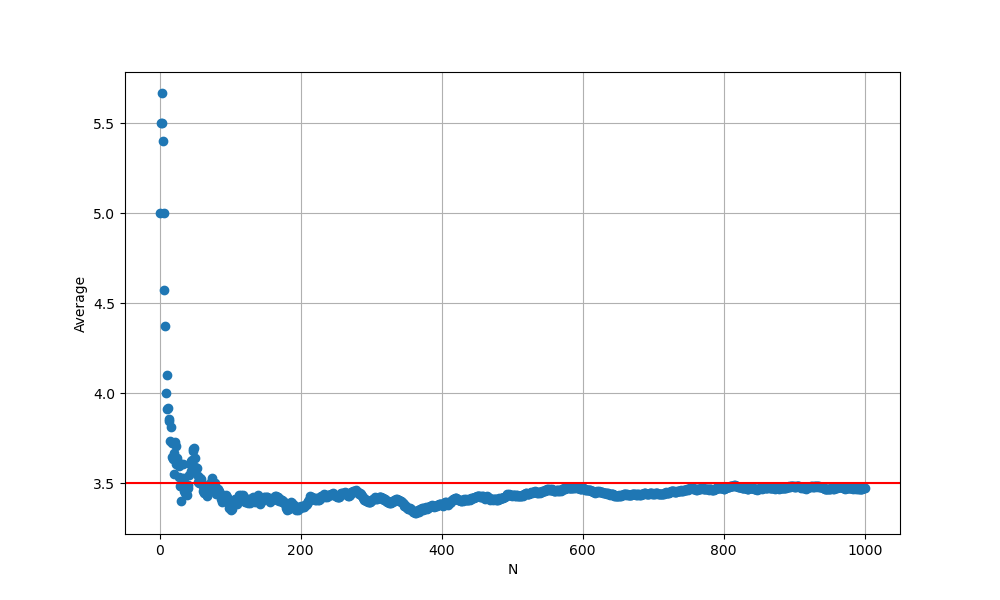
\includegraphics[width=\textwidth]{my_plot1-3.png}
  \label{f1}
  \caption{実験結果のグラフは、課題1-1で作った関数を参照}
\end{figure}
さいころの目を確率変数$X$とし、確率変数の期待値を$E[]$とする.さいころの期待値は以下の式で表せる.
\begin{align*}
  E[X] &= \frac{{1+2+3+4+5+6}}{6} \\[8pt]
  &= \frac{21}{6} \\[8pt]
  &= \frac{7}{2} \\[8pt]
  &= 3.5
  \label{e1}
\end{align*}
\begin{equation}
  平均値:3.53
\end{equation}
$1000$回さいころの目をふった平均値は図(1)の通りになる.
平均値が$n$の値が大きくになるにつれ$3.5$にちかずいていることがわかり、今回の実験で妥当な値が出ている.
\newpage
\section*{課題1-A}
\section*{実験の説明}
課題1-3 において各目 $i=1,2,...,1000  $の出る確率 $p_i$ が次のように偏っていたとする.$p_1 = p_3 =
p_5 = 1/9, p_2 = p_4 = p_6 = 2/9$. このとき,課題1-3 の結果がどう変わるかをグラフを作成して示し、その結果から考察を行う.
\section*{実験結果}
\begin{figure}[tb]
  \centering
  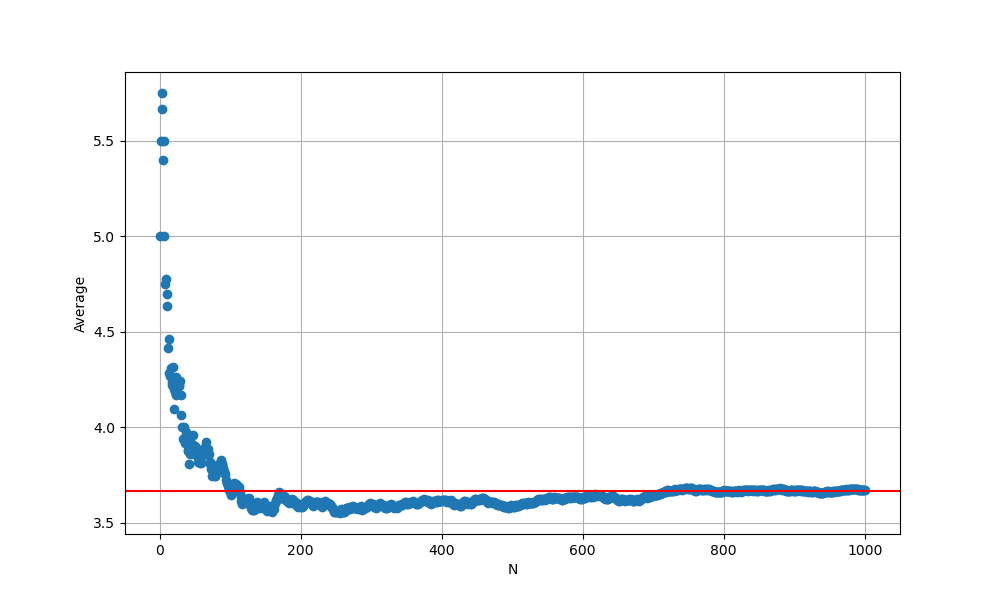
\includegraphics[width=\textwidth]{my_plot1-A.png}
  \label{f2}
  \caption{実験結果のグラフは、課題1-1で作った関数を参照}
\end{figure}

各目の出る確率が $p_1 = p_3 = p_5 = 1/9$ および $p_2 = p_4 = p_6 = 2/9$ の場合、各目が出る確率 $P(i)$ は以下のように表される.
\begin{equation}
  P(1) = P(3) = P(5) = \frac{1}{9}\\
  P(2) = P(4) = P(6) = \frac{2}{9}
\end{equation}
期待値$E$を計算するには以下のようになる.
\begin{align*}
  E &= \sum_{i=1}^{6} i \cdot P(i) \\[8pt]
  &= 1 \cdot \left(\frac{1}{9}\right) + 2 \cdot \left(\frac{2}{9}\right) + 3 \cdot \left(\frac{1}{9}\right) + 4 \cdot \left(\frac{2}{9}\right) + 5 \cdot \left(\frac{1}{9}\right) + 6 \cdot \left(\frac{2}{9}\right) \\[8pt]
  &= \frac{1}{9} + \frac{4}{9} + \frac{3}{9} + \frac{8}{9} + \frac{5}{9} + \frac{12}{9} \\[8pt]
  &= \frac{1 + 4 + 3 + 8 + 5 + 12}{9} \\[8pt]
  &= \frac{11}{3} \\[8pt]
  &= 3.67
\end{align*}
実験で得られた値は以下のとおりである.
\begin{equation}
  平均値:3.67
\end{equation}
となり、有効数値三桁では十分な精度である.
また図(2)からも理論値に知数いていることが分かる.
\section*{おわりに}
今回の実験ではたくさんのソースコードを作り、様々なライブラリなどを制作した.課題の目標であった、実践的なコーディング能力上昇に大きく貢献したと思う.
課題が複数ある慣れない形式ではあったが、それぞれについて適切な考察を行えたと思う.
\newpage
\section*{課題2-1}
\section*{実験の概要}
円周率の近似をモンテカルロ法を用いて求める.どのようにして円周率$\pi$が求まる火をいかに示す.\\
区間 $[0,1)$ の乱数の組 $(r_1,r_2)$ を独立に $n$個生成する.
一辺が$1cm$の正方形の中に半径$1cm$の円が四等分されたものがあるとする.
生成した乱数の組がその扇内にいくつ存在するかを調べ、その個数を総数で割ると、扇形の面積の近似値が出る.
半径$1$円の扇形の面積の$\frac{1}{4}$は$(\frac{\pi}{4})$となるので$4$倍することで、円周率$\pi$の近似値が得られる.
\section*{実験結果}
\begin{figure}[tb]
  \centering
  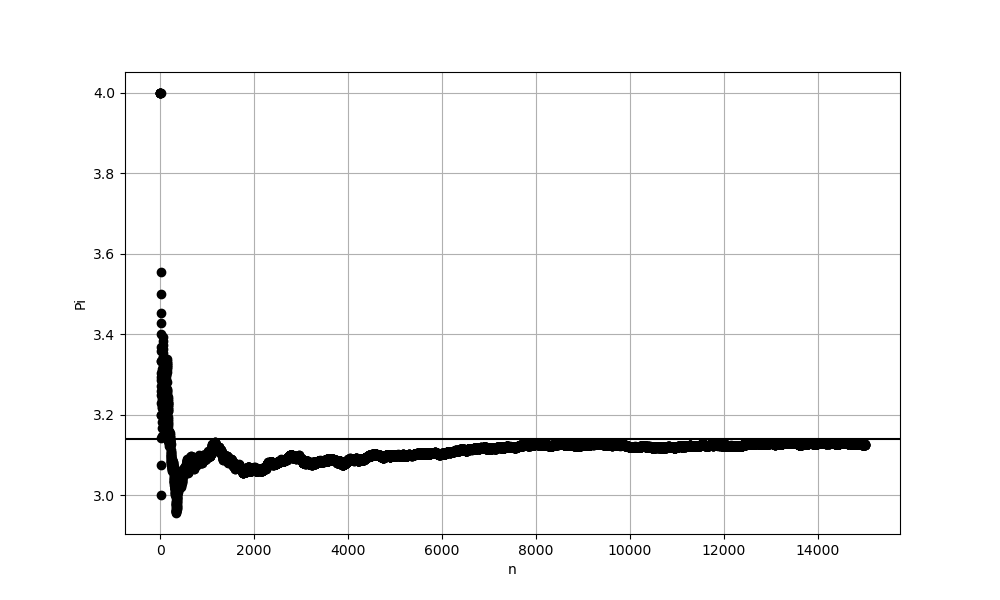
\includegraphics[width=\textwidth]{my_plot2-1.png}
  \label{f1}
  \caption{実験結果のグラフは、課題1-1で作った関数を参照}
\end{figure}
実験の概要で説明した方法で得られた$\pi$の近似値が縦軸とし、$n$の要素数を横軸に示す.
今回は$n = 15000$で実験を行った.$n = 15000$で実験を行った結果の最終的な近似値は$3.1267$となった.
グラフから$n = 8000 $あたりから近似値がずれてきていることが分かる.
\section*{考察}
今回の円周率の近似の結果はあまり正確なものではなかった.この理由として考えられるのは乱数が一様に生成されなかったことが考えられる.
今回の実験で、再現性を持たせるためにシードを学習番号に固定したが乱数に偏りを持たせてしまった可能性がある.
テストとして、シードを固定せずに実験を行った場合、$n = 10000$の時点で有効数字4桁で円周率と近似値が一致した.
より正確な近似値を得るためにはそれに適した一様な乱数を生成することが重要だろう.

\newpage
\section*{実験2-2}
1回の試行結果が確率変数$X_n$によって表される()した実験を繰り返す.
その結果において、$X_n$の(平均値)を$m$と表すとき、どんなに小さな$h(h>0)$であっても$n$が大きければ以下が成り立つ.
\[
P\left(\left|\frac{X_1 + X_2 + \ldots + X_n}{n} - m\right| \geq h\right) \rightarrow 0 \quad (1)
\]
この法則を適用して課題2-1を説明すると,確率変数 $X_1$ は1回の実験で円周の内側に入る事象 $A$ が起これば1,事象 $A$ が起こらない(円周の外側に入る)場合は0をとるものとする.このときそれぞれの事象が起こる確率は
\[
P(X_n = 1) = \frac{\pi}{4}, \quad P(X_n = 0) = \frac{3\pi}{4}  \quad (2)
\]
となるため,$m$ は以下のように計算できる.
\[
m = 1 \cdot P(X_n = 1) + 0 \cdot P(X_n = 0) = \frac{\pi}{4} \quad (3)
\]

この実験を何回も繰り返すことで確率変数 $X_1, X_2, \ldots$ を得ることができる.$n$ 回までの試行で事象 $A$ が起こる回数は $X_1 + X_2 + \ldots + X_n$ に等しいので,大数の法則に当てはめると
\[
P\left(\left|\frac{X_1 + X_2 + \ldots + X_n}{n} - \frac{\pi}{4}\right| \geq h\right) \rightarrow 0 \quad (4)
\]
となる.つまり,$\frac{X_1 + X_2 + \ldots + X_n}{n}$ は $n \rightarrow \infty$ のとき$1$に確率収束するため円周率を求めることが可能となる。

\newpage
\section*{実験2ー3}
\section*{実験の概要}
今回の実験ではモンティホール問題をシミュレーションする.モンティホール問題には以下のステップがある.
\begin{enumerate}
  \item 3つのドアがあり、各ドアの後ろには1つの賞品が隠れている.
  \item 参加者は最初に1つのドアを選ぶ.
  \item ホスト(モンティ・ホール)は、参加者が選んだドア以外の2つのドアのうち、1つを開けて、その後ろに賞品がないことを示す.
  \item 参加者には、最初に選んだドアを変更するか、そのままにするかの選択肢が与えられる。
\end{enumerate}
モンティホール問題はこのステップ4の時点で、ドアを変更するかどうかで商品の当たる確率がどのように変化するかについての問題である.
変更する場合と変更しない場合でシミュレーションを行い、当選する確率を確かめる.
\section*{実験結果}
\begin{figure}[tb]
  \centering
  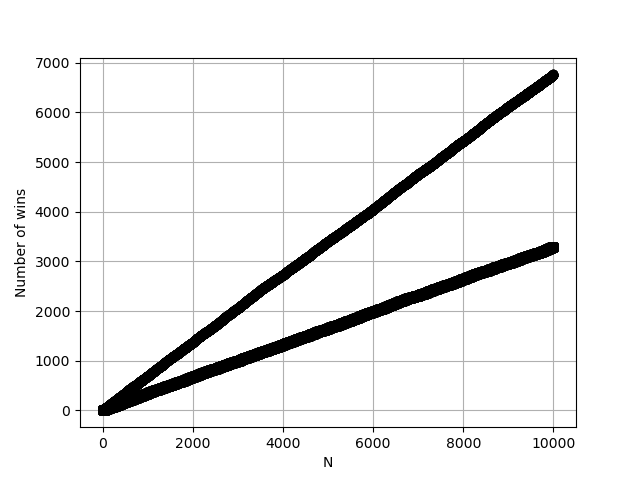
\includegraphics[width=\textwidth]{my_plot2-3.png}
  \label{f4}
  \caption{実験結果のグラフは、課題1-1で作った関数を参照}
\end{figure}
グラフから変更するのとしないので大きな差があることが分かる.
変更したほうがより当選回数が多いことが分かる.
変更をした場合の当選回数は、変更をしない場合の当選回数と比べ2倍大きくなっていた.
\section*{考察}
モンティホール問題はいくつかのステップを踏んでいるのでわかりずらいところがあるように思われる.
ドアの数が1000個で998個のドアを開けて残った1つと、自分が選んだ1では当たる確率が違うの感覚としてもわかるだろう.

\newpage

\section*{課題3-1}
\section*{実験の概要}
$500$円で購入できるお菓子の特典でブロマイドカードが1枚もらえる.特典のカードは通常版と特別版の 2
種類で,それぞれの出る確率は $\frac{1}{2}$ とする.$n$人のグループで特別版のカードを全員が入手するために必要な
予算について考える.ここで,各消費者は特別版を引くまで購入を繰り返し,特別版を一度引いた時点で購入
をやめることとする.また,お菓子は無限にあるとする.この手順を n 人全員が行ったとき,入手した全ブ
ロマイドカードのうち特別版の比率がどうなるかをシミュレーションする.
\section*{実験の結果}
\begin{figure}[tb]
  \centering
  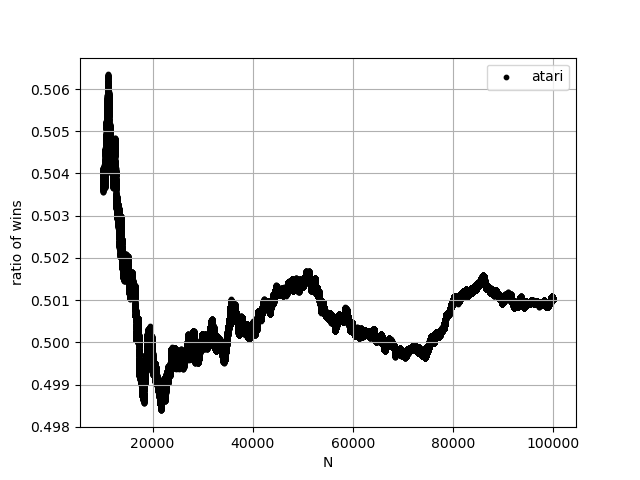
\includegraphics[width = \textwidth]{my_plot_3_1_ratio.png}
  \caption{横軸はグループの人数、縦軸は当たった確率を表す.}
  \label{f5}
\end{figure}
\begin{equation}
  あたり:0.501\\
  はずれ:0.499\\
  平均消費金額:998
\end{equation}
\begin{figure}[tb]
  \centering
  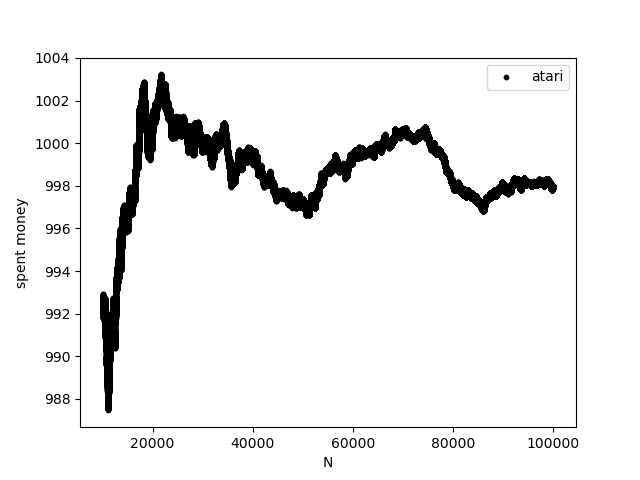
\includegraphics[width = \textwidth]{my_plot_3_1_average.png}
  \label{f6}
  \caption{横軸はグループの人数、縦軸は平均消費金額を表す.}
\end{figure}

\section*{考察}
図5より、特別ブロマイドカードの当選確率がおおよそ0.5に収束していることが分かる.
これは、あたり、はずれが出る確率と一致している.課題の指定により有効数字3桁で行った結果、誤差が$0.01$であった.
当たりが出る確率$p=0.5$と設定しているため、この結果は妥当な結果であるといえる.
理論的に、平均消費金額がどのようになるかを知るためには、期待値を計算する必要がある.
1人の特別版ブロマイドカードが当たるまでの消費金額の期待値を$E$とすると以下の式により求めることができる.

\begin{align*}
  E &= \sum_{i=1}^{\infty} 500 \left(\frac{1}{2}\right)^n\\[8pt]
  &= 500 + 500 \cdot \frac{1}{2} + 500 \cdot \left(\frac{1}{2}\right)^2 + \ldots \\[8pt]
  &= 1000
\end{align*}

以上の式から理論的には、平均消費金額が1000円になるはずである.今回の実験で得られた値は998円となっており2ずれているがこれは誤差の範囲出ある.
この実験結果から、特別版ブロマイドカードを出すためには平均1000円必要であることが分かった.\\
図(5)、図(6)ともに値にふり幅があるがこれは疑似乱数の偏りによる可能性がある.
\newpage
\section*{課題3-2}
\section*{実験の概要}
課題 3–1 の状況において,特別版と通常版の出る確率がそれぞれ 0.1 と 0.9 だった場合,特別版の比率と消
費者の平均使用金額はどうなるかをシミュレーションする.
\section*{実験結果}
\begin{figure}[tb]
  \centering
  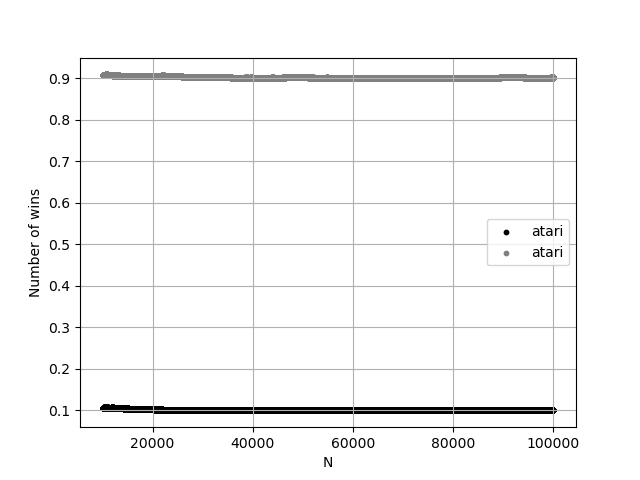
\includegraphics[width = \textwidth]{my_plot3-2_ratio.png}
  \label{f11}
  \caption{横軸はグループの人数、縦軸は当たる比率を表す.黒の点は当たる確率が0.1灰色の点が当たる確率が0.9の時である.}
\end{figure}
\begin{figure}[tb]
  \centering
  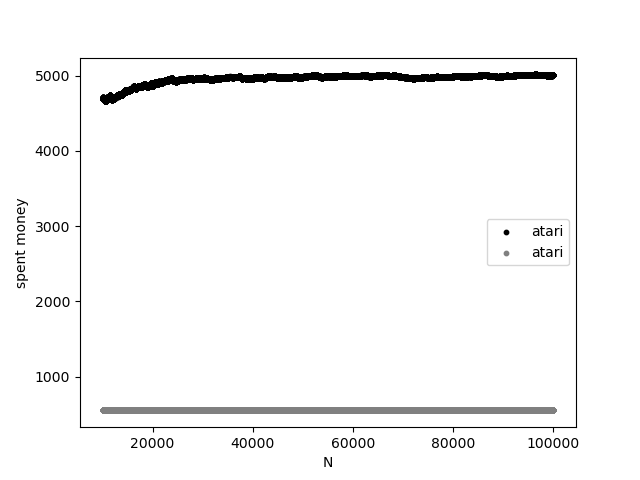
\includegraphics[width = \textwidth]{my_plot_3_2_average.png}
  \label{f12}
  \caption{横軸はグループの人数、縦軸は平均消費金額を表す.黒の点は当たる確率が0.1灰色の点が当たる確率が0.9の時である.}
\end{figure}
\begin{equation}
  当たる確率が0.1の時\\
  あたり:0.100\\
  はずれ:0.900\\
  平均消費金額:4992\\
  当たる確率が0.9の時\\
  あたり:0.900\\
  はずれ:0.100\\
  平均消費金額:555\\
\end{equation}
\section*{考察}
特別版が出る確率を$0.1, 0,9$でシミュレーションを行うと大きな差がみられた.
まず、特別版が当たる確率は設定した、$0.1,0.9$にちかずいた.これは、課題3-1デモ見られた傾向なので妥当な結果であるといえる.
また、平均消費金額はおよそ9倍ほどの差が出た.当たる確率が違うことによって、10回中1回ほど当たる場合と10回ほど9回当たる場合があるので、この結果は妥当である.
また、平均消費金額と当たりはずれの比率の倍率がそれぞれ同じなのは今回正しくシミュレーションを行うことができたことを裏付けているだろう.
\newpage
\section*{実験3-3}
\section*{実験の概要}
課題 3–1 の状況において,消費者1人あたり購入に使える予算が2千円だった場合,つまり各消費者が4個までしか購入することができないという制限がある場合を考える.この場合,特別版の比率と消費者の平均
使用金額はどうなるかをシミュレーションせよ.
\section*{実験結果}
\begin{figure}[tb]
  \centering
  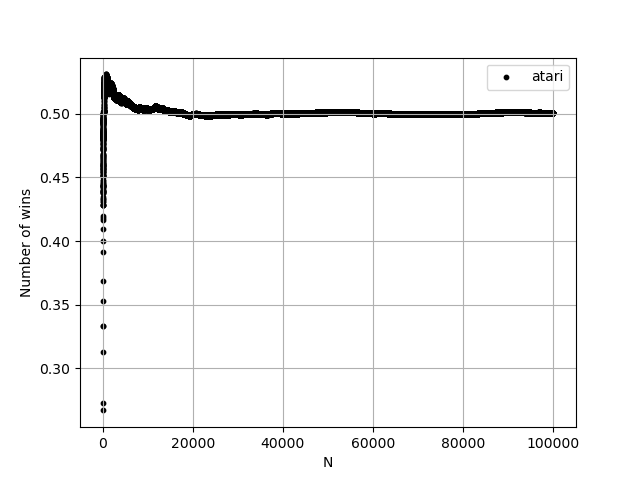
\includegraphics[width = \textwidth]{my_plot_3_3_ratio.png}
  \label{f7}
  \caption{横軸はグループの人数、縦軸は特別版ブロマイドカードが当たった比率を表す.}
\end{figure}
\begin{figure}[tb]
  \centering
  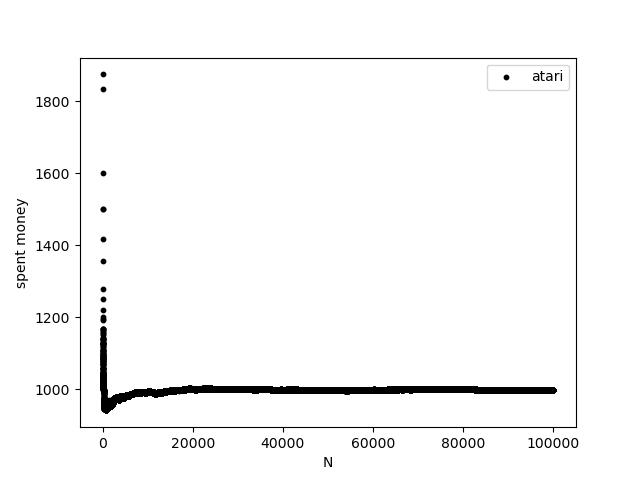
\includegraphics[width = \textwidth]{my_plot_3_3_average.png}
  \label{f8}
  \caption{横軸はグループの人数、縦軸は平均消費金額を表す.}
\end{figure}
\begin{equation}
  あたり:0.501\\
  はずれ:0.499\\
  平均消費金額:936
\end{equation}
\section*{考察}
結果から、消費する金額に予算を考慮しても当たりはずれの比率に変動は見られなかった.
今回は消費者が$4$個までしか買えないという想定で行ったが、当たる確率は$\frac{1}{2}$であり、4回連続ではずれる確率は$\frac{1}{16}$であることから、当たりはずれの比率に対して、有意な差を生まなかったことが考えられる.
課題3-1と比べて、比率に関しては有意な差がみられなかった一方で、平均消費金額はおよそ50円ほど差がある.課題1では、1人の購入上限がないため、ずっとはずれを引き続け消費金額を挙げる固体が存在することが示唆される.
それに対し、今回は購入の戸数に対して、制限をかけたため、2000円以上一人が消費することがないことから、平均消費金額が下がったのではなかと思われる.
\section*{総合の考察}
今回の実験では疑似乱数を用いて、確率的な実験を行った.実験を行う前に、自分で仮説を立てながら行っていたがおおよそ自分の仮設通りの結果となった.
今回の実験のようにプログラミングを行って実際に確率の計算を行う手法は具体的な値を求めたいときに有効であると思う.
例えば、課題3-3の場合、平均消費金額は課題3-1に比べて下がった.これは私が立てていた仮説と一致するものだが、どのくらい下がるのかなどを数学的に求めるのは困難である.そのため今回のようにシミュレーションを行うことが有効であると思った.
\bibliography{reference}
\bibliographystyle{junsrt} 

\newpage
\section*{課題3-A}
\section*{実験の概要}

課題3–1で行った500円のお菓子によるシミュレーションにおいて,消費者数を n = 10,000 人とし,お
菓子 1 個につき企業の利益が 20 円だったとする.次の2つのそれぞれの場合において,特別版のブロマイド
カードが出る確率を変化させたときの,消費者の平均使用金額及び企業の利益をシミュレーションせよ.な
お,お菓子は無限にあるとする.
\begin{enumerate}
  \item 各消費者は特別版を引くまで購入を繰り返し,特別版を一度引いた時点で購入をやめる.
  \item 各消費者に購入上限額が設定されている場合.ここでは,n = 10, 000 人の消費者のうち,購入上限額
  が 500 円の消費者を 5,000 人,1,000 円の消費者を 3,000 人,2,000 円の消費者を 1,500 人,3,000 円
  の消費者を 500 人と設定せよ.
\end{enumerate}
\section*{実験結果}
\begin{figure}[tb]
  \centering
  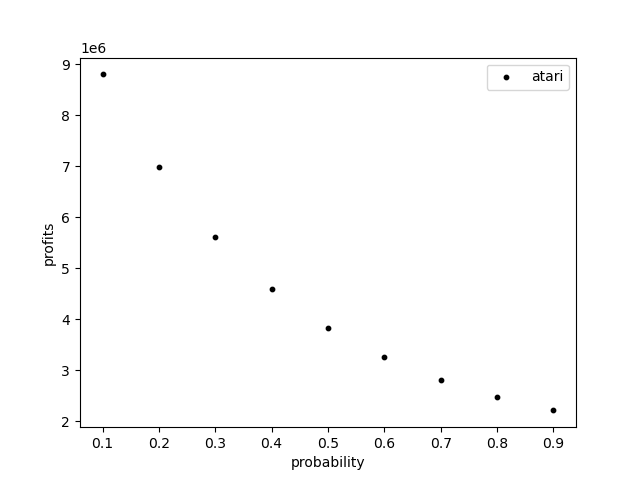
\includegraphics[width = \textwidth]{my_plot_3_A_profits.png}
  \label{f9}
  \caption{横軸は特別版ブロマイドが当たる確率、縦軸は消費者1人につき会社が得られる利益を表す.}
\end{figure}
\begin{figure}[tb]
  \centering
  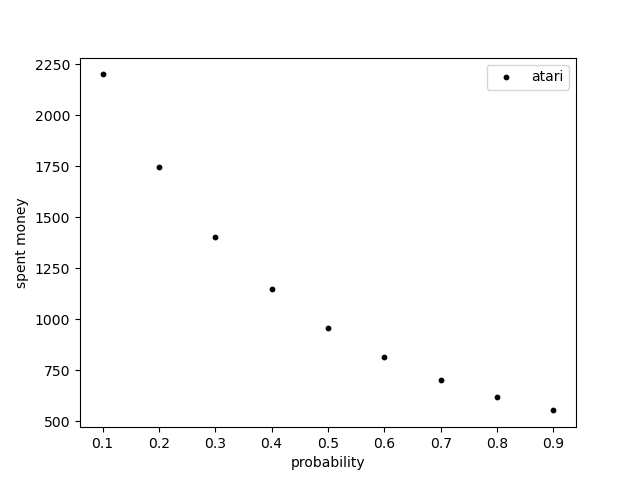
\includegraphics[width = \textwidth]{my_plot_3_A_average.png}
  \label{f10}
  \caption{横軸は特別版ブロマイドが当たる確率、縦軸は平均消費金額を表す.}
\end{figure}
図9と図10は同じ傾向を見せた.特別版ブロマイドが当たる確率をあげていくと消費者1人につき会社が得られる利益と、平均消費金額はともに下がっていった.
\section*{考察}
特別版ブロマイドが当たる確率をあげると、当たるまでに購入する回数が減り、平均消費金額が下がることが予測される.また、購入あれた商品の数が減れば必然的に、利益も下がっていった.
会社側としてより利益をあげるには、利益率と、値段、当たる確率の塩梅を考える必要がある.
\newpage
\section*{課題4-1}
\section*{実験の概要}
中心極限定理を確認するシミュレーションを作成し,実行する.
\begin{enumerate}
  \item 平均0,分散1の正規分布に従う乱数$X_i (i = 1, . . . , n)$ を独立に n 個生成し,n 個の平$\overline{X}(n) = \frac{(\sum_{i=1}^{n} X_i)}{n}$ を求める関数 normal$\_$rand を作成する
  \item  $n$個の$X$の平均$\overline{X}_n$ を求める試行を $m$ 回行い,$m$ 個の $\overline{X}(n)$ を求める.
\end{enumerate}
\section*{実験結果}
\begin{figure}[tb]
  \centering
  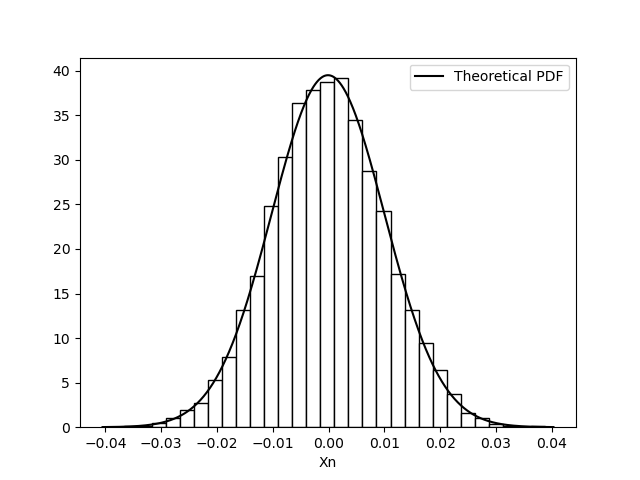
\includegraphics[width = \textwidth]{my_plot_4_1.png}
  \label{f11}
  \caption{横軸は$X_n$の値、縦軸は標本数を表す.}
\end{figure}
\begin{itemize}
  \item $m:10$
    \begin{itemize}
      \item 平均値: $0.0000022$
      \item 分散: $0.0000000$
    \end{itemize}
  \item $m:100$
    \begin{itemize}
      \item 平均値: $0.0000219$
      \item 分散: $0.0000000$
    \end{itemize}
  \item $m:1000$
    \begin{itemize}
      \item 平均値: $0.000219$
      \item 分散: $0.0000004$
    \end{itemize}
  \item $m:10000$
    \begin{itemize}
      \item 平均値: $0.00219$
      \item 分散: $-0.0000000$
    \end{itemize}
\end{itemize}
\section*{考察}
図(13)より、課題で生成した乱数から計算した$\overline{X}_n$が正規分布に従っていることが分かる.
理論的な正規分布の曲線にしたがっているのは中心極限定理から説明することができる.
中心極限定理では、 $m$を大きくすれば、標本の平均値は平均(元の集団の平均値)、分散(元の集団の分散を標本の数で割った値)の正規分布に従う.
今回 $m= 10000$でプロットしたが、正規分布に従ってプロットされていることから、$m=10000$は中心極限定理を示すのに十分大きな値であると言える.
$\overline{X}(n)$の平均値は理論とは異なった結果を示した.$X$の平均$\overline{X}_n$が$m$こ生成される平均は、$0$になるはずであるが、今回は$0$とは違う値に近づいた.
この値は$m$の値が大きくなるほど$0$に近づくはずであるが今回の結果では、逆に離れていった.これはシミュレーションの方法に何か間違いがあるか、疑似乱数がうまく作動していないことが考えられる.
平均値の値とは違い、分散の値は理論値に近い値となった.今回の実験では、分散の値は$0$になるはずであり、実験の結果でも$0$に非常に近い値となった.
\newpage
\section*{課題4-2}
\section*{実験の概要}
第 1 回目のサイコロのシミュレーションを用いて中心極限定理を確認する.
\begin{enumerate}
  \item サイコロを$n$回独立に振り,$n$個の出た目の平均$\overline{Y}_n$を求める.
  \item $n$個の出た目の平均$\overline{Y}_n$を求める試行を$m$回行い,$m$個の$\overline{Y}_n$ を求める.
\end{enumerate}
\section*{実験結果}
\begin{figure}[tb]
  \centering
  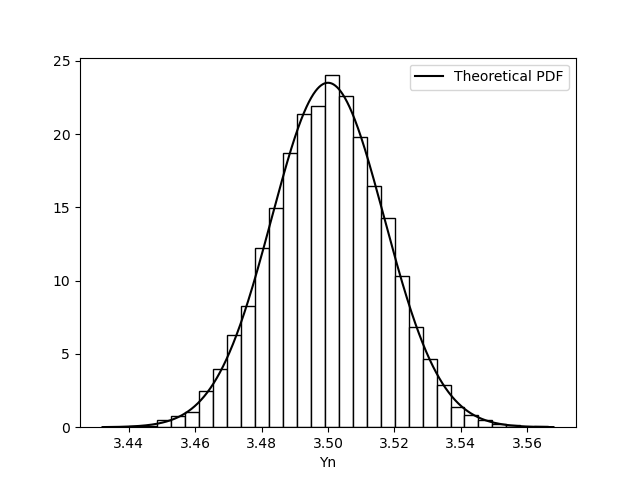
\includegraphics[width = \textwidth]{my_plot_4_2.png}
  \label{f12}
  \caption{横軸は$X_n$の値、縦軸は標本数を表す.}
\end{figure}
\begin{table}[h]
  \centering
  \begin{tabular}{cccc}
    \toprule
    $m$ & 平均値 & 分散 \\
    \midrule
    10    & 3.49096 & 0.0001866 \\
    100   & 3.49924 & 0.000303313 \\
    1000  & 3.50022 & 0.000282348 \\
    10000 & 3.49998 & 0.000284963 \\
    \bottomrule
  \end{tabular}
  \caption{実験結果}
  \label{tab:experiment_results}
\end{table}
\section*{考察}
今回の実験での平均と分散の理論値は、$3.5$と$0$である.表(1)より、平均値は$m$が大きくなるほど、$3.5$に近づいていることが分かる.
さらに、分散も$m$が大きくなるにつれ、理論値に近づいている.ただ$m=1000$の時と、$m=10000$の時ではあまり差がない.これは$m=1000$でも十分正確な値が出ることを示している.
図(14)から、課題で生成した乱数から計算した$\overline{Y}_n$が正規分布に従っていることが分かる.中心極限定理は$m \rightarrow \infty$の時に、理論的な分布に従うことを示すが、$m=10000$でもある程度の近似であれば十分であることが分かった.

\section*{実験4-A}
\section*{実験の概要}
母集団がベルヌーイ分布(二項分布)であることを想定して中心極限定理を確認する.ここでは,ベルヌーイ分布として第$1$回目の課題1-2 で作成したコイン投げを $p = 0.3$ としてシミュレーションを実行する.
\begin{enumerate}
  \item コイン投げを$n$回独立に行い,$n$ 回のうち,表が出た割合 $\overline{P}_n$ を求める.
  \item $\overline{P}_n$ を求める試行を $m$ 回行い,$m$ 個の $\overline{P}_n$ を求める.
\end{enumerate}
\section*{実験結果}
\begin{figure}[tb]
  \centering
  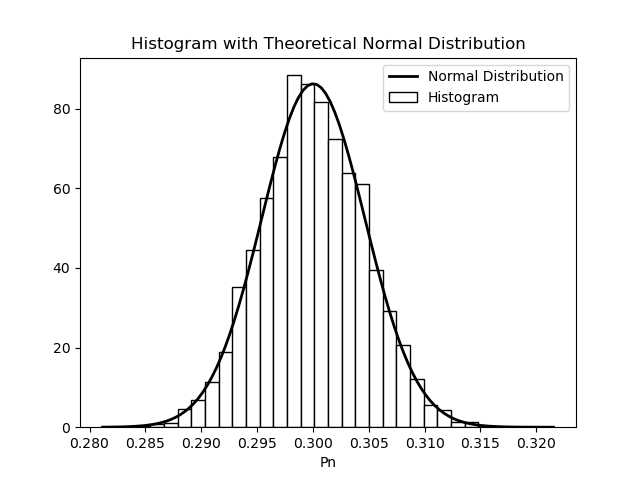
\includegraphics[width = \textwidth]{my_plot_4_A.png}
  \label{f13}
  \caption{横軸は$P_n$の値、縦軸は標本数を表す.}
\end{figure}
\begin{table}[h]
  \centering
  \caption{結果のまとめ}
  \begin{tabular}{cccc}
      \toprule
      $m$ & 平均値 & 分散 \\
      \midrule
      10    & 0.29783   & 0.0000238 \\
      100   & 0.2998530 & 0.0000183 \\
      1000  & 0.3001655 & 0.0000212 \\
      10000 & 0.3000320 & 0.0000214 \\
      \bottomrule
  \end{tabular}
\end{table}
\section*{考察}  
図(15)からわかるように今回の実験では理論に近い分布となった.$P_n$が$0.295$から$0.300$までのところに理論的な標本数より少し標本数が多くなったところがあるが、これは疑似乱数の生成の誤差によって収まる範囲である.
また、平均値と分散の理論的な値に非常に近い結果となった.
今回は表が当たる確率$p = 0.3$としていることから、理論的な平均値は$0.3$となる.表2から$m$の値が大きくなるほどに平均値が$0.3$に近づいている.
分散の理論値は今回も$0$となるはずであり、すべての$m$の値に対して、理論値と近い値をとっている.ただ、$m$の増加とともに、理論値に近づく傾向はない.これは、$P_n$を生成する乱数が理想的な分布をなしていることから、$m = 10$でも十分理論値に近いことが原因として考えられる.
以上より母集団がベルヌーイ分布の場合でも中心極限定理が成立することが確認できた.


\newpage
\section*{付録}
今回の課題に使用したソースコードを以下に示す.
\begin{cppcode}
  #include<iostream>
#include<random>
using namespace std;

//ランド関数を作る
void rnd_exp(double A[], int n){
    random_device rd;
    mt19937 gen(rd());
    uniform_real_distribution<double> distribution(0.0,1.0);
    for(int i = 0; i < n; i++){
        double r = distribution(gen);
        A[i] = r;
    }
}
int main(){
    int n = 1000;
    double A[n];
    rnd_exp(A,n);
    double sum1 = 0;
    double sum2 = 0;
    for(int i = 0; i < n ; i++){
        sum1 += A[i];
        sum2 += A[i] * A[i];
    }
    double ave = sum1 / n;
    cout << "平均値: " << sum1/n << endl;
    cout << "分散: " << sum2/n - ave*ave << endl;
    return 0;
}
\end{cppcode}
\begin{cppcode}
  #include<iostream>
#include<random>
using namespace std;

//ランド関数を作る
void rnd_exp(double A[], int n){
    random_device rd;
    mt19937 gen(rd());
    uniform_real_distribution<double> distribution(0.0,1.0);
    for(int i = 0; i < n; i++){
        double r = distribution(gen);
        A[i] = r;
    }
}

int main(){
    int n = 1000;
    double A[n];
    rnd_exp(A,n);
    double p1 = 0.3;
    double p2 = 0.5;
    double p3 = 0.7;
    double R1, R2, R3;
    R1 = 0;
    R2 = 0;
    R3 = 0;
    for(int i = 0; i < n; i++){
        if(A[i] < p1){
        }
        else if(p1 <= A[i] && A[i] <= p2 ){
            R1++;
        }
        else if(p2 < A[i] && A[i] <= p3){
            R1++;
            R2++;
        }
        else if(p3 < A[i]){
            R1++;
            R2++;
            R3++;
        }
    }
    cout << "p = 0.3の時" << R1/n << endl;
    cout << "p = 0.5の時" << R2/n << endl;
    cout << "p = 0.7の時" << R3/n << endl;

    return 0;
}
\end{cppcode}
\begin{cppcode}
  #include<iostream>
#include<random>
#include<fstream>
using namespace std;

//ランド関数を作る
void rnd_exp(double A[], int n){
    random_device rd;
    mt19937 gen(rd());
    uniform_real_distribution<double> distribution(0.0,1.0);
    for(int i = 0; i < n; i++){
        double r = distribution(gen);
        A[i] = r;
    }
}
int GenDice(){
    random_device rd;
    mt19937 gen(rd());
    uniform_int_distribution<int> distribution(1, 6);
    return distribution(gen);
}

int main(){
    ofstream of("DiceAverage.csv");
    of << "N,Average" <<endl; 
    int n = 1000;
    double A[n];
    rnd_exp(A,n);
    double sum = 0;

    for(int i = 0; i < n; i++){
        sum += GenDice();
        of << i+1 << "," << sum/(i+1) << endl;
    }
    cout << sum/n << endl;
    return 0;
}
\end{cppcode}
\begin{cppcode}
  #include<iostream>
#include<random>
#include<fstream>
using namespace std;

//ランド関数を作る
void rnd_exp(double A[], int n){
    random_device rd;
    mt19937 gen(rd());
    uniform_real_distribution<double> distribution(0.0,1.0);
    for(int i = 0; i < n; i++){
        double r = distribution(gen);
        A[i] = r;
    }
}
int GenDice(){
    random_device rd;
    mt19937 gen(rd());
    uniform_int_distribution<int> distribution(1, 9);
    int a = distribution(gen);
    if(a == 7) a = 2;
    if(a == 8) a = 4;
    if(a == 9) a = 6;
    return a;
}

int main(){
    ofstream of("DiceAverage1-A.csv");
    of << "N,Average" <<endl; 
    int n = 1000;
    double A[n];
    rnd_exp(A,n);
    double sum = 0;

    for(int i = 0; i < n; i++){
        sum += GenDice();
        of << i+1 << "," << sum/(i+1) << endl;
    }
    return 0;
}
\end{cppcode}
\begin{cppcode}
  #include<iostream>
#include<random>
#include<math.h>
#include<iomanip>
#include<fstream>
using namespace std;
void rnd_exp(double A[], double B[], int n){
    int rd = 22140003;
    mt19937 mt(rd);
    uniform_real_distribution<double> distribution(0.0,1.0);
    for(int i = 0; i < n; i++){
        double r = distribution(mt);
        double s = distribution(mt);
        A[i] = r;
        B[i] = s;
    }
}
int main(){
    ofstream of("kadai_2_1.csv");
    of << "n,pi"<<endl;
    int n = 15000;
    double R1[n], R2[n];
    rnd_exp(R1,R2,n);
    int count = 0;
    for(int i = 0; i< n;i++){
        double r;
        r = pow(R1[i],2) + pow(R2[i],2);
        if(r < 1.000)count++;
        double a = i + 1.0;
        of << i+1 << "," << fixed << setprecision(4) << 4.0*(count/(a)) << endl;
    }
    double N = n + 0.0;
    double rat = count/N;
    cout << fixed << setprecision(4) << 4*rat << endl;
    return 0;
}
\end{cppcode}
\begin{cppcode}
  #include<iostream>
#include<random>
#include<fstream>
using namespace std;
void rnd_exp(int A[], int B[], int n){
    int rd = 22140003;
    mt19937 mt(rd);
    uniform_int_distribution<int> distribution(1,3);
    for(int i = 0; i < n; i++){
        int r = distribution(mt);
        int s = distribution(mt);
        A[i] = r;
        B[i] = s;
    }
}
//bool MontyHallNOCHANGE(){}
int main(){
    ofstream of("kadai_2_3.csv");
    of << "n,nochange,change" << endl;
    //1を正解のボックスとする.
    int n = 10000;
    int A[n], B[n];
    int change = 0;
    int Nochange = 0;
    rnd_exp(A,B,n);
    for(int j = 0;j<n;j++){
        if(A[j]==1)Nochange++;
        if(B[j]==2 || B[j] == 3)change++;
        of << j + 1 << ","<< Nochange<<","<< change << endl;
    }
    cout << "変更なし" << Nochange/(n+0.0) << endl;
    cout << "変更あり" << change/(n+0.0) << endl;
    return 0;
    
}
\end{cppcode}
\begin{cppcode}
  #include<iostream>
#include<random>
#include<cmath>
#include<vector>
#include<iomanip>
#include<fstream>
using namespace std;

//make random numbers in an array


int main(){
    //set random numbers
    int n = 100000;
    //set probability
    double p = 0.5;
    int seed = 22140003;
    mt19937 mt(seed);
    uniform_real_distribution<double> distribution(0.0, 1.0);
    //set variable
    int count_loop = 0;
    int count_tousen = 0;
    //create a file for ratio
    ofstream of("kadai_3_1_ratio.csv");
    of << "n,tousen" << endl;

    //create a file for  average spent
    ofstream file("kadai_3_1_average_expenditure.csv");
    file << "n,average" << endl;


    while(1){
        double prob = distribution(mt);
        if(prob > p){
            count_tousen++;
        }
        else if(prob < p){
        }
        count_loop++;
        if(10000 < count_tousen && count_tousen < 100000 ){
            double N = n;
            double tousen = count_tousen;
            double hazure = count_loop - count_tousen;
            of << count_tousen << "," << tousen/count_loop << endl; 
            file << count_tousen << "," << (count_loop*500.0) / count_tousen << endl;
        }
        if(count_tousen == n)break;
    }
    double N = n;
    double tousen = count_tousen;
    double hazure = count_loop - count_tousen;
    cout << fixed << setprecision(3) <<  "あたり:" << tousen/count_loop << "はずれ:" << hazure/count_loop << endl;
    cout <<fixed << setprecision(0)<< "平均消費金額" << (count_loop*500) / N<< endl;
    return 0;
}
\end{cppcode}
\begin{cppcode}
  #include<iostream>
#include<random>
#include<cmath>
#include<vector>
#include<iomanip>
#include<fstream>
using namespace std;

//make random numbers in an array


int main(){
    //set random numbers
    int n = 100000;
    //set probability
    double p = 0.9;
    int seed = 22140003;
    mt19937 mt(seed);
    uniform_real_distribution<double> distribution(0.0, 1.0);
    //set variable
    int count_loop = 0;
    int count_tousen = 0;
    double spnetmoney = 0;
    int stop_hazure = 0;
    //create a file for ratio
    ofstream of("kadai_3_2_ratio.csv");
    of << "n,tousen" << endl;

    //create a file for  average spent
    ofstream file("kadai_3_2_average_expenditure.csv");
    file << "n,average" << endl;

    
    while(1){
        double prob = distribution(mt);
        spnetmoney += 500;
        count_loop++;
        if(prob > p){
            count_tousen++;
        }
        if(10000 < count_loop && count_loop < 100000 ){
            double N = n;
            double tousen = count_tousen;
            double hazure = count_loop - count_tousen;
            of << count_loop << "," << tousen/count_loop << endl; 
            file << count_loop << "," << (count_loop*500.0) / count_tousen << endl;
        }
        if(count_loop - count_tousen == n){
            stop_hazure = count_loop;
        }
        if(count_tousen == n)break;
    }
    double N = n;
    double tousen = count_tousen;
    double hazure = count_loop - count_tousen;
    cout << "当たる確率が0.1の場合" << endl;
    cout << fixed << setprecision(3) <<  "あたり:" << tousen/count_loop << "はずれ:" << hazure/count_loop << endl;
    cout <<fixed << setprecision(0)<< "平均消費金額" << (count_loop*500) / N<< endl;
    cout << "当たる確率が0.9の場合" << endl;
    cout << fixed << setprecision(3) <<  "あたり:" << hazure/count_loop << "はずれ:" << tousen/count_loop << endl;
    cout <<fixed << setprecision(0)<< "平均消費金額" << (stop_hazure*500) / N<< endl;

    return 0;
}
#include<iostream>
#include<random>
#include<cmath>
#include<vector>
#include<iomanip>
#include<fstream>
using namespace std;


int main(){
    //set random numbers
    int n = 100000;
    //set probability
    double p = 0.5;
    int seed = 22140003;
    mt19937 mt(seed);
    uniform_real_distribution<double> distribution(0.0, 1.0);
    //set variable
    int count_loop = 0;
    int count_tousen = 0;
    int count_people = 0;
    int countfour = 0;
    double spentmoney = 0;
    //create a file for ratio
    ofstream of("kadai_3_3_ratio.csv");
    of << "n,tousen" << endl;

    //create a file for  average spent
    ofstream file("kadai_3_3_average_expenditure.csv");
    file << "n,average" << endl;


    while(1){
        spentmoney += 500.0;
        countfour++;
        count_loop++;
        double prob = distribution(mt);
        if(prob > p){
            count_tousen++;
            countfour = 0;
            count_people++;
            of << count_people << "," << count_tousen / double(count_loop) << endl;
            file << count_people <<"," << spentmoney/ double(count_tousen) << endl;

        }
        else if(countfour == 4 && prob < p){
            countfour = 0;
            count_people++;
            of << count_people << "," << count_tousen / double(count_loop) << endl;
            file << count_people <<"," << spentmoney/ double(count_tousen) << endl;
        }
        if(count_people == n)break;
    }
    double N = n;
    double tousen = count_tousen;
    double hazure = count_loop - count_tousen;
    cout << fixed << setprecision(3) <<  "あたり:" << tousen/count_loop << "はずれ:" << hazure/count_loop << endl;
    cout <<fixed << setprecision(0)<< "平均消費金額" <<  spentmoney/ n<< endl;
    return 0;
}
#include<iostream>
#include<random>
#include<cmath>
#include<vector>
#include<iomanip>
#include<fstream>
using namespace std;

int main(){

    //set probability
    int seed = 22140003;
    mt19937 mt(seed);
    uniform_real_distribution<double> distribution(0.0, 1.0);

    //create csv files
    ofstream of("kadai_3_A_average_expenditure.csv");
    ofstream file("kadai_3_A_profits.csv");

    //header
    of << "prob,average" << endl;
    file << "prob,profit" << endl;

    for(double p = 0.1; p<= 0.9; p += 0.1){
        //set variables
        int count_people = 0;
        double price = 500;
        int n = 100000;
        double prof = 20;
        double reven = 0;
        int tousen = 0;
        int count = 0;
        int count_loop = 0;
        double spentmoney = 0;
        //main loop
        while(1){
            spentmoney += 500;
            count_loop++;
            reven += prof;
            if(0 <= count_people && count_people < 5000){
                if(p > distribution(mt)){
                    tousen++;
                    count_people++;
                }
                else{
                    count_people++;
                }
            }
            else if (5000 <= count_people && count_people < 8000){
                count++;
                if(p > distribution(mt)){
                    tousen++;
                    count_people++;
                    count = 0;
                }
                else if(count == 2){
                    count_people++;
                    count = 0;
                }
            }
            else if(8000 <= count_people && count_people < 9500){
                count++;
                if(p > distribution(mt)){
                    tousen++;
                    count_people++;
                    count = 0;
                }
                else if(count == 4){
                    count_people++;
                    count = 0;
                }
            }
            else{
                count++;
                if(p > distribution(mt)){
                    tousen++;
                    count_people++;
                    count = 0;
                }
                else if(count == 6){
                    count_people++;
                    count = 0;
                }
            }
            if(count_people == n){
                break;
            }
        }

        of << p << "," << spentmoney / count_people << endl;
        file << fixed << setprecision(1) << p << "," << reven << endl;
        }
    return 0;
}
\end{cppcode}
\begin{cppcode}
#include<iostream>
#include<random>
#include<fstream>
#include<iomanip>
#include<cmath>
using namespace std;

double normal_rand(int n){
    random_device rd;
    mt19937 mt(rd());
    //set mean and median
    double mean = 0.0;
    double var = 1.0;
    //define normal distribution
    normal_distribution<double> dist(mean,var);

    double sum = 0;
    //generate random number for n times
    for(int i =0; i < n; i ++){
        sum += dist(mt);
    }
    return sum / n;
}
int main(){
    //create a file
    ofstream of("kadai_4_1.csv");
    of << "Xn" << endl;
    //set variables
    int n = 10000;
    //
    for(int m = 10; m<= 10000; m *= 10){
       double sum = 0;
       double sum2 = 0;
       for(int i = 0;i < m; i++){
        double rnd = normal_rand(n);
        sum += rnd;
        sum2 += pow(rnd,2);
        if(m == 10000){
            of << rnd << endl;
        }
       }
       cout << "m:" << m << endl;
       cout << fixed << setprecision(7) << "平均値" << sum / m << endl;
       cout << "分散" << (sum2 / m) - pow((sum/m),2) << endl;
    }


    return 0;
}
#include<iostream>
#include<random>
#include<fstream>
using namespace std;

double rnd_int(int n){
    random_device rd;
    mt19937 mt(rd());
    //define normal distribution
    uniform_int_distribution<int> dist(1,6);
    double sum = 0;
    //generate random number for n times
    for(int i =0; i < n; i ++){
        sum += dist(mt);
    }
    return sum / n;
}
int main(){
    int n = 10000;
    //file
    ofstream of("kadai_4_2.csv");
    of << "Yn" << endl;
    for(int m = 10; m <= 10000; m *= 10){
        double sum = 0;
        double sum2 = 0;
        for(int i = 0; i < m; i++){
            double Y = rnd_int(n);
            sum += Y;
            sum2 += pow(Y,2);
            if(m == 10000){
                of << Y << endl;
            }
        }
        cout << "m:" << m << endl;
        cout << "平均値" << sum / m << endl;
        cout <<"分散" << (sum2/m) - pow(sum/m,2) << endl;
    }
    return 0;
}

#include<iostream>
#include<random>
#include<fstream>
#include<iomanip>
using namespace std;

double rnd_coin(int n){
    random_device rd;
    mt19937 mt(rd());
    //define normal distribution
    uniform_real_distribution<double> dist(0.0,1.0);
    double sum = 0;
    double p =0.3;
    int head=0;
    int loop=0;;
    while(1){
        loop++;
        if(p > dist(mt)){
            head++;
        }
        if(loop == n){
            break;
        }
    }
    return double(head) / n;
}
int main(){
    int n = 10000;
    //file
    ofstream of("kadai_4_A.csv");
    of << "Pn" << endl;
    for(int m = 10; m <= 10000; m *= 10){
        double sum = 0;
        double sum2 = 0;
        for(int i = 0; i < m; i++){
            double P = rnd_coin(n);
            sum += P;
            sum2 += pow(P,2);
            if(m == 10000){
                of << P << endl;
            }
        }
        cout << "m:" << m << endl;
        cout << "平均値" << sum / m << endl;
        cout << fixed <<setprecision(7) << "分散" << (sum2/m) - pow(sum/m,2) << endl;
    }
    return 0;
}

\end{cppcode}
\newpage
\bibliography{reference}
\bibliographystyle{junsrt} 

(参考文献.\cite{example} などを参考に,bib ファイルの使い方はウェブなどで勉強すること.)

\end{document}